\documentclass[runningheads,a4paper,11pt]{report}

\usepackage{algorithmic}
\usepackage{algorithm} 
\usepackage{array}
\usepackage{amsmath}
\usepackage{amsfonts}
\usepackage{amssymb}
\usepackage{amsthm}
\usepackage{caption}
\usepackage{comment} 
\usepackage{epsfig} 
\usepackage{fancyhdr}
\usepackage[T1]{fontenc}
\usepackage{geometry} 
\usepackage{graphicx}
\usepackage[colorlinks]{hyperref} 
\usepackage[latin1]{inputenc}
\usepackage{multicol}
\usepackage{multirow} 
\usepackage{rotating}
\usepackage{setspace}
\usepackage{subfigure}
\usepackage{todonotes}
\usepackage{url}
\usepackage{verbatim}
\usepackage{xcolor}
\usepackage[super]{nth}

\geometry{a4paper,top=3cm,left=2cm,right=2cm,bottom=3cm}

\pagestyle{fancy}
\fancyhf{}
\fancyhead[LE,RO]{Sense}
\fancyhead[RE,LO]{Bogdan-Daniel B\u{a}l\u{a}nescu}
\fancyfoot[RE,LO]{ITSG 2019-2020}
\fancyfoot[LE,RO]{\thepage}

\renewcommand{\headrulewidth}{2pt}
\renewcommand{\footrulewidth}{1pt}
\renewcommand{\headrule}{\hbox to\headwidth{%
  \color{lime}\leaders\hrule height \headrulewidth\hfill}}
\renewcommand{\footrule}{\hbox to\headwidth{%
  \color{lime}\leaders\hrule height \footrulewidth\hfill}}

\hypersetup{
pdftitle={artTitle},
pdfauthor={name},
pdfkeywords={pdf, latex, tex, ps2pdf, dvipdfm, pdflatex},
bookmarksnumbered,
pdfstartview={FitH},
urlcolor=cyan,
colorlinks=true,
linkcolor=red,
citecolor=green,
}
% \pagestyle{plain}

\setcounter{secnumdepth}{3}
\setcounter{tocdepth}{3}

\linespread{1}

% \pagestyle{myheadings}

\makeindex


\begin{document}

\begin{titlepage}
\sloppy
\begin{center}
BABE\c S BOLYAI UNIVERSITY, CLUJ NAPOCA, ROM\^ ANIA

FACULTY OF MATHEMATICS AND COMPUTER SCIENCE

\vspace{5cm}

\Huge \textbf
{
Face expression recognition for social good \\
- road to smart acting -
}

\vspace{1cm}

\normalsize -- ITSG report --

\end{center}


\vspace{4cm}

\begin{flushleft}
\Large{\textbf{Teacher}}\\
Laura Dio\textcommabelow{s}an\\
Intelligent Tools for Social Good
\end{flushleft}

\begin{flushright}
\Large{\textbf{Author}}\\
Bogdan-Daniel B\u{a}l\u{a}nescu\\
Software Engineering, 258-1
\end{flushright}

\vspace{3cm}

\begin{center}
2019
\end{center}

\end{titlepage}

\pagenumbering{gobble}

\begin{abstract}
	This paper studies the problem of Face Expression Recognition (REC) in an attempt to build a tool that helps novice actors better analyze their performance and get real-time feedback to improve. Starting from the Convolutional Neural Network proposed in \cite{Arriaga17}, and trained on the FER-2013 emotion database, this paper slightly improves the 66\% learning accuracy of the proposed algorithm to 68\%. An application, Acting Mirror, is proposed and presented in the last part of the paper, as well as all the results and comparisons with other state of the art research. In the conclusion, we see that the current study of FER is facing a few issues we raise from our study and we propose a few improvement action points that could be tackled in the future.
\end{abstract}


\tableofcontents

\newpage

%\listoftables
%\listoffigures
%\listofalgorithms

\newpage

\setstretch{1.5}



\newpage

\pagenumbering{arabic}


 


\chapter{Introduction}
\label{chapter:introduction}

\section{What? Why? How?}
\label{section:what}

For novice actors, it is often hard to control their emotions and to express what is on their script well, so the need for an expert to be with them when they rehearse is needed. A tool that would give them feedback in real-time may just make their start easier. It could be there for them anytime and for free, rather than hiring an expert to watch them rehearse.\\
This paper addresses this problem by proposing a tool able to recognize emotions from real-time video footage or photos.

\begin{itemize}
	\item \textbf{\emph{What?}} The problem of Face Expression Recognition (FER) is a classification problem which has received an important amount of attention in the last decade with various approaches such as the feature-based Tree-Augmented-Naive Bayes (TAN) classifier, Local Binary Patterns (LBP) classifier, Support Vector Machines and numerous Neural Networks based approaches. \cite{Caleanu13}
	\item \textbf{\emph{Why?}} The importance of FER is present in a variety of domains, such as: psychology, neuroscience and even philosophy. Science today still cannot explain for sure where do emotions come from or if emotions are the ones driving our decisions or not. With this in mind, an approach that involves artificial intelligence capable of classifying emotions from photos would prove useful until other studies provide a better or a more accessible solution.
	\item \textbf{\emph{How?}} In this paper, we present an artificially intelligent solution to recognizing emotions from pictures. From a dataset of pictures labeled with emotions we will train a model able to classify emotions.
\end{itemize}

[The work of next laboratories will add here: 
A short discussion of how it fits into related work in the area. Summary of the basic results and conclusions.]


\section{Paper structure and original contribution(s)}
\label{section:structure}

[Should present here this information when improvement of the algorithm is done: The research presented in this paper advances the theory, design, and implementation of the proposed alogrithm.]

The main contribution of this report is to present an intelligent algorithm for solving the problem of Face Expression Recognition.

The second contribution of this report consists of building an intuitive, easy-to-use and user friendly software application. Our aim is to build an application that will help novice actors to better analyze their facial expressions and get real-time feedback while rehearsing.
Main feature present in the application (and other possible improvements):
\begin{itemize}
	\item \textbf{\emph{Main feature:}} The user shall be able to record themselves in real-time and see their emotions in the video.
	\item \textbf{\emph{Future improvement:}} The user shall be able to provide an acting script with labeled emotions on certain sections of text.
	\item \textbf{\emph{Future improvement:}} The user shall receive real-time feedback based on the labeled script when they make a mistake.
\end{itemize}

The third contribution of this thesis consists of providing a comparison between state of the art results in FER and the proposed algorithm.

[Should be present in the next laboratories: The present work contains $xyz$ bibliographical references and is structured in five chapters as follows.]

In the second chapter we will take a look at a formal introduction of our FER problem and weight the advantages and disadvantages of using AI to solve it.

The third chapter will describe the state of the art in FER.

In the the fourth chapter we will further detail our proposed approach to solving the problem. 

[Short placeholder here, until we reach detailing the third chapter: (dataset with pictures and labels (emotion) -> new dataset facial points (features) and labels (emotion) -> model to solve the problem)]

The fifth chapter will present a comparison for the chosen methodology, data and results between two different approaches to solving this problem (ours and one more).

The final chapter will present our conclusions and future work to be done regarding this problem and application.

\chapter{Scientific Problem}
\label{section:scientificProblem}
++

\section{Problem definition}
\label{section:problemDefinition}

For people pursuing their hobby of acting, it might be hard to hire an expert while rehearsing or even coming to terms with the tight schedule of a hard working day and a few minutes of spare time to rehearse a play. The need for a tool that would assist people when rehearsing, giving them feedback about their facial expressions in real life, arises and we pursue to deliver such an application.\\
The solution to such a tool is required to use an intelligent algorithm, because as far as we know, there exist no other methodologies for approaching this problem and it also falls into the category of complex problems that may be more easily solved using a neural network or other intelligent algorithms.\\

Advantages of solving the problem with an intelligent algorithm:
\begin{itemize}
	\item it is much faster to reach a solution than proceeding with finding a non-intelligent algorithm to solve it
 	\item it may be impossible to solve it using non-intelligent algorithms due to the vast lack of knowledge in the area of human emotions
\end{itemize}

Disadvantages of solving the problem with an intelligent algorithm:
\begin{itemize}
	\item it may require a lot of work in training and retraining models until we reach a suitable (efficient and accurate) model to solve the problem
	\item it is impossible to reach, using A.I., a solution which has a 100\% accuracy
\end{itemize}

\pagebreak
Short description of our initial approach:
\begin{itemize}
	\item From an existing dataset, FER-2013, which contains 35,887 48x48 pixel grayscale labeled images, 80\% of pictures were used for training, while the remaining 20\% were used for validation of the algorithm.
	\item The model was trained locally using Keras on an i7-7500u and an NVIDIA Quadro M520 1GB. It took a little bit over 2 hours of training and the achieved validation accuracy was 65\%. While doing the validation precision/accuracy test, it takes approximately 1 milliseconds for the model to analyze a 48x48 pixel grayscale image.
\end{itemize}


\chapter{State of art/Related work}
\label{chapter:stateOfArt}


\section{State of the Art}
\label{section:soa}

In this section we present a few methods utilized in order to solve the Facial Expression Recognition (FER) problem.

\textbf{First}, we will take a look at \cite{Tarnowski17}, where the problem is solved using k-NN (Nearest Neighbors) and MLP (Multilayer Perceptron).
\begin{itemize}
	\item \textbf{\emph{What kind of data did they use?}} Coefficients describing elements of facial expressions (as features) and a range of seven emotional states (as labels). The emotional states detected are: neutral, joy, sadness, surprise, anger, fear, disgust. The images they used were from the KDEF database.
	\item \textbf{\emph{How does their model(s) work?}} Using Microsoft Kinect 3D for face modeling, they were able to extract 3D models of the face as 3D points, but Kinect 3D also can extract Action Units (AC) based on those points, which basically represent certain features of the face. Choosing 6 of those Action Units (upper lip raising, jaw lowering, lip stretching, lowering eyebrows, lip corner depressing, outer brow raising) they were able to train a 3-NN and an MLP classifier in order to solve the FER problem.
	\item \textbf{\emph{What were their results?}} They tested the models for two cases: a) subject-dependent and b) subject-independent. For the 3-NN classifier, they got around 95-96\% accuracy and for the MLP algorithms the results were around 75-76\%. \todo{please indicate the dataset used for obtaining these performances - SOLVED - KDEF}
\end{itemize}

\textbf{Second}, let us look at \cite{Samadiani19}, where three significant challenges in FER are discussed: illumination variation, head pose and subject-dependence. We shall focus on the ones that target visual-only databases.
\begin{itemize}
	\item \textbf{\emph{What about illumination variation?}} The paper compares different approaches to FER, like SVM (Support Vector Machines) with 31-50\% accuracy, Deep Networks with 48-96\% accuracy and KNN with 92-96\% accuracy. The most utilized dataset was the CK+ dataset. The paper suggests using Fast Fourier Transform and Contrast Limited Adaptive Histogram Equalization (FFT+CLAHE) to overcome poor lighting conditions, among other techniques.
	\item \textbf{\emph{What about subject-dependece?}} Subject-dependence means the model is only able to recognize the expressions of the faces it trained with. The paper proposes a solution, where geometric face features were extracted, and using a part-based hierarchical recurrent neural network (PHRNN) to model the facial morphological variations, a multi-signal convolutional neural network (MSCNN) to find the spatial features of face, an accuracy of around 98.5\% can be achieved. The used dataset was CK+.
\end{itemize}

\textbf{Last, but not least}, let us take a look at \cite{Burkert16}, a practical approach using a Convolutional Neural Network (CNN).
\begin{itemize}
	\item \textbf{\emph{What kind of data did they use?}} The used datasets were MMI and CKP and they recognized emotions from the following list: anger, sadness, disgust, happiness, fear and surprise.
	\item \textbf{\emph{How does their model(s) work?}} Their proposed model is independent from any other third-party feature extraction frameworks and it performs better than the previously proposed CNN models, with an accuracy of 93-99\% on the above mentioned datasets. Their model begins with a convolutional layer over the input and then filtering max pooling layer, before entering two fully connected layers (comprised of convolution + pooling, then convolution + convolution, then concatenation and pooling), after which they classify the images with softmax layer.
	\item \textbf{\emph{What were their results?}} Their accuracy was around 99\%.
\end{itemize}


So far, we have seen three great state of the art examples. One which uses an third-party framework to manipulate the dataset so that the model can be a very simple one to train, like a 3-NN. Another set of examples where top state of the art models were presented and certain impediments were discussed (such as illumination variation and subject-dependency) and one other example which is independent on any other third-party framework in its learning, while still achieving good results.


\section{Useful Tools}
\label{section:ut}


Now, let us give a list of useful tools to use when developing intelligent applications:
\begin{itemize}
	\item Tensorflow, is a Python framework for building machine learning models. A javascript version, Tensorflow.js, also exists.
	\item Tensorflow Lite, a framework for building machine learning models compatible with portable devices (i.e. mobile phones).
	\item ML Kit for Firebase, a mobile SDK that empowers mobile applications with Google's machine learning packages. It is also possible to host one's own machine learning model in Firebase (have not experienced with this yet).
	\item YOLO: Real-Time Object Detection, is a state of the art object detection system, but which can also be trained for a different purpose. It is open source and written in C++.
	\item fastAI, is a Python framework for buildign machine learning models. Also comes with pre-trained models for certain problems.
\end{itemize}


\chapter{Proposed approach}
\label{chapter:proposedApproach}

\section{Algorithm description}
\label{section:ad}

Starting from the Convolutional Neural Network proposed in \cite{Arriaga17} (and which is inspidred by the Xception \cite{Chollet16} architecture), and presented in the following figure (see Figure \ref{cnnModel}), our approach is to use an already existing algorithm capable of classifying emotions and integrate it in an easy to use application in order to help novice actors get real-time feedback about their performance.

\begin{figure}[htbp]
\begin{center}
	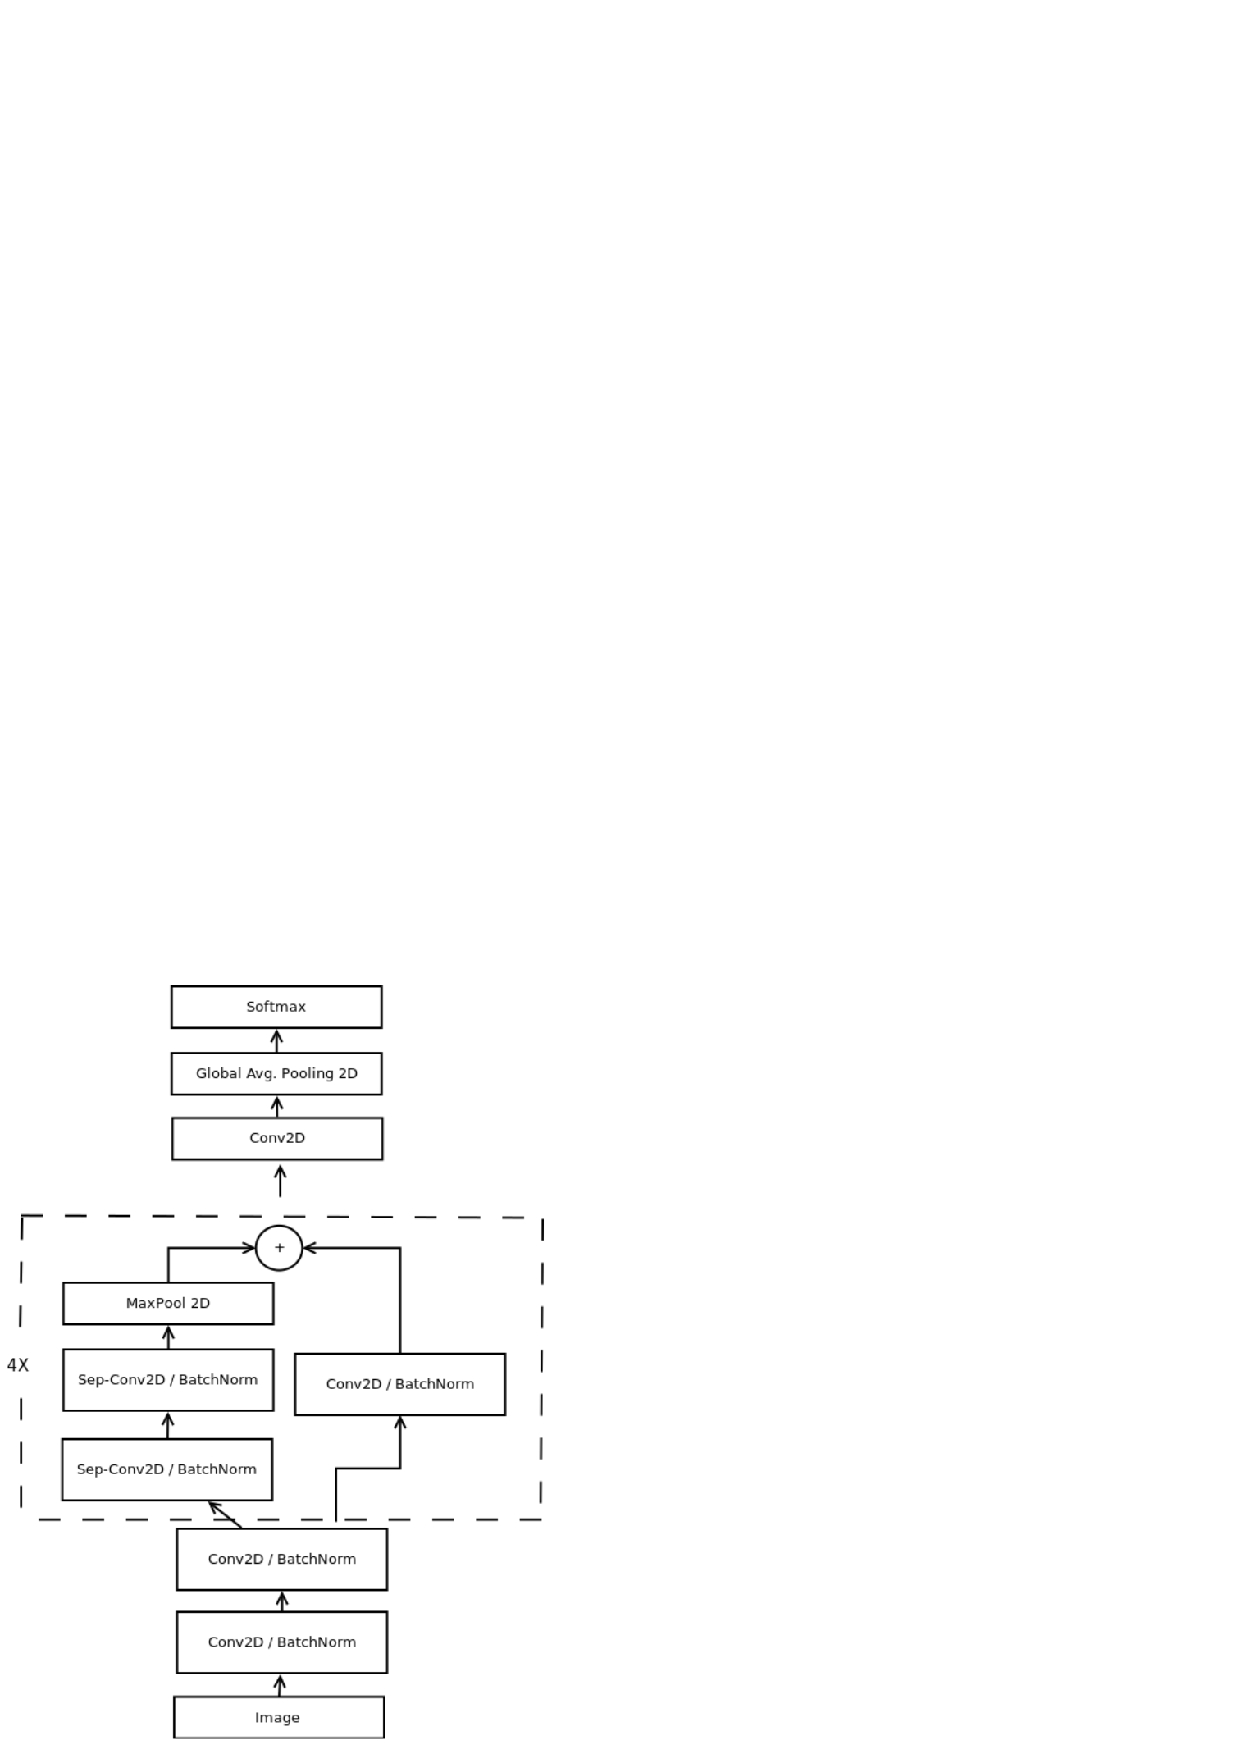
\includegraphics[scale=0.37]{Fig/cnnModel.pdf}
	\caption{\cite{Arriaga17} proposed model for real-time classification of emotions}
	\label{cnnModel}
\end{center}
\end{figure}

We used the FER-2013 emotion database, which contains 35.887 48x48 pixel grayscale labeled images with the following emotions: (0=Angry, 1=Disgust, 2=Fear, 3=Happy, 4=Sad, 5=Surprise, 6=Neutral). Initially, we performed 7 training trials, one using original approach proposed in \cite{Arriaga17}, and then by changing the learning rate and the loss function during training.\\
For the original approach proposed in \cite{Arriaga17}, we achieved a 65\% validation accuracy over the FER-2013 database (using all the 35.887 images), and a 76\% accuracy over the CK+ database using the same model trained on the FER-2013 database.\\
From our other approaches, the fifth one achieved a 64\% validation accuracy over the FER-2013 dabase (using only 28.709 of the images), and a 79\% accuracy over the CK+ database using the same model trained on the FER-2013 database.


\chapter{Application (numerical validation)}
\label{chapter:application}

For the proposed algorithm, our approach was to perform several training sessions, with different inputs for the independent variables and see how they affect the learning. The reason for this, was to find a way to improve the accuracy of the model. As will be related in the following section, we have played around with the learning rate and with the loss function of the algorithm. Unfortunately, what we have found is that the algorithm reaches a plateou of learning from which it cannot escape, thus, the accuracy of the model being around 65\%, almost like what was achieved in \cite{Arriaga17}.

\section{Methodology}
\label{section:meth}
In this chapter, we analyze the achieved results for the proposed algorithm using the following approach. We present the training dataset and independent variables, a plot of the achieved training results and how well it fairs against the CK+ dataset, presenting the precision for each emotion separately.\\
The independent variables we are experimenting with are the learning rate, and the loss function.\\
The dependent variables will be the weights of the model.\\
For our first attempt, we have used the whole FER-2013 dataset, and obtained a validation accuracy of 65\%, and for the next attempts we shall only use the Training pictures from the FER-2013 dataset, and it will also enable us to compute the precision for the Public Test set and Private Test set of the FER-2013 dataset.\\ \todo{here, the classifier was trained on FER and test on CK+ or it was trained from scratch by using CK+ data? - SOLVED - it was trained only on FER and tested on CK+}
For comparison purposes between our models trained on the FER-2013 dataset, we also compute the precision for each model against the CK+ emotion dataset and present the results here. \\
\textbf{Side note:} for the first five trials, we test the model on the CK+ dataset as it is, but after that, we realised we forgot to filter the CK+ dataset through the Haarscade Frontal Face Detector model provided by OpenCV. We came back, and redid the tests on the as such \textbf{processed} CK+ dataset.\\
\textbf{Note:} From here on, when we refer to testing our model against the CK+ dataset, we mean to test it against the processed CK+ dataset, unless stated otherwise.

\section{Obtained results}
\label{section:or}
\underline{\textbf{\emph{The first trial:}}}
\begin{itemize}
	\item \textbf{Dataset}: FER-2013, 35.887 images, split into 80\% training and 20\% validation.
	\item \textbf{Input size}: [1, 48, 48, 1] grayscale pixel images. Each pixel, a value between [0, 255].
	\item \textbf{Output size}: [1, 7] tensor containing the percentages for each label.
	\item \textbf{Loss function}: Categorical Crossentropy.
	\item \textbf{Optimizer}: Adam.
	\item \textbf{Learning rate}: 0.1.
	\item \textbf{Batch size}: 32.
	\item \textbf{Epochs}: 110.
	\item \textbf{Training metric}: Accuracy.
\end{itemize}
The result was a training validation accuracy of 65\%, and a 76\% accuracy on the CK+ dataset.
\begin{figure}[htbp]
\begin{center}
	\includegraphics[scale=0.8]{Fig/fer_training_35k.pdf}
	\caption{Training results using all the 35.887 images in the FER-2013 emotion dataset}
	\label{fer_training_35k}
\end{center}
\end{figure}

\begin{table}[htbp]
	\caption{The precisin results against the CK+ dataset for the first training trial}
	\label{fer_training_35k_ckp}
		\begin{center}
			\begin{tabular}{p{110pt}p{110pt}c}
				\textbf{Emotion}& \textbf{Precision}& \textbf{No. of pictures} \\
				\hline\hline
				Angry& 0.16& 45 \\
				Disgust& 0.00& 59 \\
				Fear& 0.03& 25 \\
				Happy& 0.68& 69 \\
				Sad& 0.12& 28 \\
				Surprise& 0.00& 83 \\
				Neutral& 0.03& 1 \\
				\hline
				Weighted Average& 0.19& 310
			\end{tabular}
		\end{center}
\end{table}

\begin{table}[htbp]
	\caption{The precisin results against the \textbf{unprocessed} CK+ dataset for the first training trial}
	\label{fer_training_35k_unprocessed_ckp}
		\begin{center}
			\begin{tabular}{p{110pt}p{110pt}c}
				\textbf{Emotion}& \textbf{Precision}& \textbf{No. of pictures} \\
				\hline\hline
				Angry& 0.30& 45 \\
				Disgust& 0.91& 59 \\
				Fear& 0.43& 25 \\
				Happy& 0.94& 69 \\
				Sad& 0.39& 28 \\
				Surprise& 0.97& 83 \\
				Neutral& 0.00& 1 \\
				\hline
				Weighted Average& 0.76& 310
			\end{tabular}
		\end{center}
\end{table}

\clearpage
\underline{\textbf{\emph{The second trial:}}}
\begin{itemize}
	\item \textbf{Dataset}: FER-2013, 28.709 images, split into 80\% training and 20\% validation.
	\item \textbf{Input size}: [1, 48, 48, 1] grayscale pixel images. Each pixel, a value between [0, 255].
	\item \textbf{Output size}: [1, 7] tensor containing the percentages for each label.
	\item \textbf{Loss function}: Categorical Crossentropy.
	\item \textbf{Optimizer}: Adam.
	\item \textbf{Learning rate}: 0.1.
	\item \textbf{Batch size}: 32.
	\item \textbf{Epochs}: 110.
	\item \textbf{Training metric}: Accuracy.
\end{itemize}
The result was a training validation accuracy of 63\%, and a 76\% accuracy on the CK+ dataset.
\begin{figure}[htbp]
\begin{center}
	\includegraphics[scale=0.8]{Fig/fer_training_28k_01.pdf}
	\caption{Training results using 28.709 images from the FER-2013 emotion dataset}
	\label{fer_training_28k_01}
\end{center}
\end{figure}

\begin{table}[htbp]
	\caption{The precisin results against the CK+ dataset for the second training trial}
	\label{fer_training_28k_01_ckp}
		\begin{center}
			\begin{tabular}{p{110pt}p{110pt}c}
				\textbf{Emotion}& \textbf{Precision}& \textbf{No. of pictures} \\
				\hline\hline
				Angry& 0.21& 45 \\
				Disgust& 1.00& 59 \\
				Fear& 0.53& 25 \\
				Happy& 0.91& 69 \\
				Sad& 0.52& 28 \\
				Surprise& 0.94& 83 \\
				Neutral& 0.00& 1 \\
				\hline
				Weighted Average& 0.76& 310
			\end{tabular}
		\end{center}
\end{table}
\begin{table}[htbp]
	\caption{The precisin results against the FER-2013 Public Test dataset for the second training trial}
	\label{fer_training_28k_01_public_test}
		\begin{center}
			\begin{tabular}{p{110pt}p{110pt}c}
				\textbf{Emotion}& \textbf{Precision}& \textbf{No. of pictures} \\
				\hline\hline
				Angry& 0.51& 467 \\
				Disgust& 0.67& 56 \\
				Fear& 0.47& 496 \\
				Happy& 0.82& 895 \\
				Sad& 0.52& 653 \\
				Surprise& 0.74& 415 \\
				Neutral& 0.55& 607 \\
				\hline
				Weighted Average& 0.62 &3589
			\end{tabular}
		\end{center}
\end{table}
\begin{table}[htbp]
	\caption{The precisin results against the FER-2013 Private Test dataset for the second training trial}
	\label{fer_training_28k_01_private_test}
		\begin{center}
			\begin{tabular}{p{110pt}p{110pt}c}
				\textbf{Emotion}& \textbf{Precision}& \textbf{No. of pictures} \\
				\hline\hline
				Angry& 0.53& 467 \\
				Disgust& 0.47& 56 \\
				Fear& 0.47& 496 \\
				Happy& 0.84& 895 \\
				Sad& 0.50& 653 \\
				Surprise& 0.74& 415 \\
				Neutral& 0.61& 607 \\
				\hline
				Weighted Average& 0.63 &3589
			\end{tabular}
		\end{center}
\end{table}
\begin{table}[htbp]
	\caption{The precisin results against the \textbf{unprocessed} CK+ dataset for the second training trial}
	\label{fer_training_28k_01_unprocessed_ckp}
		\begin{center}
			\begin{tabular}{p{110pt}p{110pt}c}
				\textbf{Emotion}& \textbf{Precision}& \textbf{No. of pictures} \\
				\hline\hline
				Angry& 0.19& 45 \\
				Disgust& 0.00& 59 \\
				Fear& 0.05& 25 \\
				Happy& 0.52& 69 \\
				Sad& 0.15& 28 \\
				Surprise& 1.00& 83 \\
				\hline
				Weighted Average& 0.43& 310
			\end{tabular}
		\end{center}
\end{table}

\clearpage
\underline{\textbf{\emph{The third trial:}}}
\begin{itemize}
	\item \textbf{Dataset}: FER-2013, 28.709 images, split into 80\% training and 20\% validation.
	\item \textbf{Input size}: [1, 48, 48, 1] grayscale pixel images. Each pixel, a value between [0, 255].
	\item \textbf{Output size}: [1, 7] tensor containing the percentages for each label.
	\item \textbf{Loss function}: Categorical Crossentropy.
	\item \textbf{Optimizer}: Adam.
	\item \textbf{Learning rate}: 0.01.
	\item \textbf{Batch size}: 32.
	\item \textbf{Epochs}: 110.
	\item \textbf{Training metric}: Accuracy.
\end{itemize}
The result was a validation accuracy of 63\%, and a 60\% accuracy on the CK+ dataset.
\begin{figure}[htbp]
\begin{center}
	\includegraphics[scale=0.8]{Fig/fer_training_28k_001.pdf}
	\caption{Training results using 28.709 images from the FER-2013 emotion dataset}
	\label{fer_training_28k_001}
\end{center}
\end{figure}

\begin{table}[htbp]
	\caption{The precisin results against the CK+ dataset for the third training trial}
	\label{fer_training_28k_001_ckp}
		\begin{center}
			\begin{tabular}{p{110pt}p{110pt}c}
				\textbf{Emotion}& \textbf{Precision}& \textbf{No. of pictures} \\
				\hline\hline
				Angry& 0.25& 45 \\
				Disgust& 0.00& 59 \\
				Fear& 0.80& 25 \\
				Happy& 0.89& 69 \\
				Sad& 0.54& 28 \\
				Surprise& 0.95& 83 \\
				Neutral& 0.00& 1 \\
				\hline
				Weighted Average& 0.60& 310
			\end{tabular}
		\end{center}
\end{table}
\begin{table}[htbp]
	\caption{The precisin results against the FER-2013 Public Test dataset for the third training trial}
	\label{fer_training_28k_001_public_test}
		\begin{center}
			\begin{tabular}{p{110pt}p{110pt}c}
				\textbf{Emotion}& \textbf{Precision}& \textbf{No. of pictures} \\
				\hline\hline
				Angry& 0.52& 467 \\
				Disgust& 0.62& 56 \\
				Fear& 0.48& 496 \\
				Happy& 0.84& 895 \\
				Sad& 0.54& 653 \\
				Surprise& 0.74& 415 \\
				Neutral& 0.55& 607 \\
				\hline
				Weighted Average& 0.63 &3589
			\end{tabular}
		\end{center}
\end{table}
\begin{table}[htbp]
	\caption{The precisin results against the FER-2013 Private Test dataset for the third training trial}
	\label{fer_training_28k_001_private_test}
		\begin{center}
			\begin{tabular}{p{110pt}p{110pt}c}
				\textbf{Emotion}& \textbf{Precision}& \textbf{No. of pictures} \\
				\hline\hline
				Angry& 0.57& 467 \\
				Disgust& 0.73& 56 \\
				Fear& 0.48& 496 \\
				Happy& 0.85& 895 \\
				Sad& 0.48& 653 \\
				Surprise& 0.76& 415 \\
				Neutral& 0.59& 607 \\
				\hline
				Weighted Average& 0.64 &3589
			\end{tabular}
		\end{center}
\end{table}
\begin{table}[htbp]
	\caption{The precisin results against the \textbf{unprocessed} CK+ dataset for the third training trial}
	\label{fer_training_28k_001_unprocessed_ckp}
		\begin{center}
			\begin{tabular}{p{110pt}p{110pt}c}
				\textbf{Emotion}& \textbf{Precision}& \textbf{No. of pictures} \\
				\hline\hline
				Angry& 0.17& 45 \\
				Disgust& 0.00& 59 \\
				Fear& 0.02& 25 \\
				Happy& 0.62& 69 \\
				Sad& 0.18& 28 \\
				Surprise& 1.00& 83 \\
				Neutral& 0.02& 1 \\
				\hline
				Weighted Average& 0.45& 310
			\end{tabular}
		\end{center}
\end{table}

\clearpage
\underline{\textbf{\emph{The fourth trial:}}}
\begin{itemize}
	\item \textbf{Dataset}: FER-2013, 28.709 images, split into 80\% training and 20\% validation.
	\item \textbf{Input size}: [1, 48, 48, 1] grayscale pixel images. Each pixel, a value between [0, 255].
	\item \textbf{Output size}: [1, 7] tensor containing the percentages for each label.
	\item \textbf{Loss function}: Mean Square Error.
	\item \textbf{Optimizer}: Adam.
	\item \textbf{Learning rate}: 0.01.
	\item \textbf{Batch size}: 32.
	\item \textbf{Epochs}: 110.
	\item \textbf{Training metric}: Accuracy.
\end{itemize}
The result were a validation accuracy of 63\%, and a 69\% accuracy on the CK+ dataset.
\begin{figure}[htbp]
\begin{center}
	\includegraphics[scale=0.8]{Fig/fer_training_28k_001_mean_square.pdf}
	\caption{Training results using 28.709 images from the FER-2013 emotion dataset}
	\label{fer_training_28k_001_mean_square}
\end{center}
\end{figure}

\begin{table}[htbp]
	\caption{The precisin results against the CK+ dataset for the fourth training trial}
	\label{fer_training_28k_001_mean_square_ckp}
		\begin{center}
			\begin{tabular}{p{110pt}p{110pt}c}
				\textbf{Emotion}& \textbf{Precision}& \textbf{No. of pictures} \\
				\hline\hline
				Angry& 0.23& 45 \\
				Disgust& 0.67& 59 \\
				Fear& 0.56& 25 \\
				Happy& 0.85& 69 \\
				Sad& 0.43& 28 \\
				Surprise& 0.96& 83 \\
				Neutral& 0.00& 1 \\
				\hline
				Weighted Average& 0.69& 310
			\end{tabular}
		\end{center}
\end{table}
\begin{table}[htbp]
	\caption{The precisin results against the FER-2013 Public Test dataset for the fourth training trial}
	\label{fer_training_28k_001_mean_square_public_test}
		\begin{center}
			\begin{tabular}{p{110pt}p{110pt}c}
				\textbf{Emotion}& \textbf{Precision}& \textbf{No. of pictures} \\
				\hline\hline
				Angry& 0.53& 467 \\
				Disgust& 0.61& 56 \\
				Fear& 0.51& 496 \\
				Happy& 0.82& 895 \\
				Sad& 0.54& 653 \\
				Surprise& 0.76& 415 \\
				Neutral& 0.53& 607 \\
				\hline
				Weighted Average& 0.63 &3589
			\end{tabular}
		\end{center}
\end{table}
\begin{table}[htbp]
	\caption{The precisin results against the FER-2013 Private Test dataset for the fourth training trial}
	\label{fer_training_28k_001_mean_square_private_test}
		\begin{center}
			\begin{tabular}{p{110pt}p{110pt}c}
				\textbf{Emotion}& \textbf{Precision}& \textbf{No. of pictures} \\
				\hline\hline
				Angry& 0.56& 467 \\
				Disgust& 0.52& 56 \\
				Fear& 0.50& 496 \\
				Happy& 0.85& 895 \\
				Sad& 0.49& 653 \\
				Surprise& 0.74& 415 \\
				Neutral& 0.58& 607 \\
				\hline
				Weighted Average& 0.63 &3589
			\end{tabular}
		\end{center}
\end{table}
\begin{table}[htbp]
	\caption{The precisin results against the \textbf{unprocessed} CK+ dataset for the fourth training trial}
	\label{fer_training_28k_001_mean_square_unprocessed_ckp}
		\begin{center}
			\begin{tabular}{p{110pt}p{110pt}c}
				\textbf{Emotion}& \textbf{Precision}& \textbf{No. of pictures} \\
				\hline\hline
				Angry& 0.13& 45 \\
				Disgust& 0.00& 59 \\
				Fear& 0.12& 25 \\
				Happy& 0.49& 69 \\
				Sad& 0.12& 28 \\
				Surprise& 1.00& 83 \\
				Neutral& 0.00& 1 \\
				\hline
				Weighted Average& 0.42& 310
			\end{tabular}
		\end{center}
\end{table}

\clearpage
\underline{\textbf{\emph{The fifth trial:}}}
\begin{itemize}
	\item \textbf{Dataset}: FER-2013, 28.709 images, split into 80\% training and 20\% validation.
	\item \textbf{Input size}: [1, 48, 48, 1] grayscale pixel images. Each pixel, a value between [0, 255].
	\item \textbf{Output size}: [1, 7] tensor containing the percentages for each label.
	\item \textbf{Loss function}: Mean Square Error.
	\item \textbf{Optimizer}: Adam.
	\item \textbf{Learning rate}: 0.1.
	\item \textbf{Batch size}: 32.
	\item \textbf{Epochs}: 110.
	\item \textbf{Training metric}: Accuracy.
\end{itemize}
The result were a validation accuracy of 64\%, and a 79\% accuracy on the CK+ dataset.
\begin{figure}[htbp]
\begin{center}
	\includegraphics[scale=0.8]{Fig/fer_training_28k_01_mean_square.pdf}
	\caption{Training results using 28.709 images from the FER-2013 emotion dataset}
	\label{fer_training_28k_01_mean_square}
\end{center}
\end{figure}

\begin{table}[htbp]
	\caption{The precisin results against the CK+ dataset for the fifth training trial}
	\label{fer_training_28k_01_mean_square_ckp}
		\begin{center}
			\begin{tabular}{p{110pt}p{110pt}c}
				\textbf{Emotion}& \textbf{Precision}& \textbf{No. of pictures} \\
				\hline\hline
				Angry& 0.21& 45 \\
				Disgust& 1.00& 59 \\
				Fear& 0.67& 25 \\
				Happy& 0.94& 69 \\
				Sad& 0.55& 28 \\
				Surprise& 0.94& 83 \\
				Neutral& 0.00& 1 \\
				\hline
				Weighted Average& 0.79& 310
			\end{tabular}
		\end{center}
\end{table}
\begin{table}[htbp]
	\caption{The precisin results against the FER-2013 Public Test dataset for the fifth training trial}
	\label{fer_training_28k_01_mean_square_public_test}
		\begin{center}
			\begin{tabular}{p{110pt}p{110pt}c}
				\textbf{Emotion}& \textbf{Precision}& \textbf{No. of pictures} \\
				\hline\hline
				Angry& 0.53& 467 \\
				Disgust& 0.56& 56 \\
				Fear& 0.48& 496 \\
				Happy& 0.84& 895 \\
				Sad& 0.56& 653 \\
				Surprise& 0.78& 415 \\
				Neutral& 0.53& 607 \\
				\hline
				Weighted Average& 0.63 &3589
			\end{tabular}
		\end{center}
\end{table}
\begin{table}[htbp]
	\caption{The precisin results against the FER-2013 Private Test dataset for the fifth training trial}
	\label{fer_training_28k_01_mean_square_private_test}
		\begin{center}
			\begin{tabular}{p{110pt}p{110pt}c}
				\textbf{Emotion}& \textbf{Precision}& \textbf{No. of pictures} \\
				\hline\hline
				Angry& 0.54& 467 \\
				Disgust& 0.62& 56 \\
				Fear& 0.47& 496 \\
				Happy& 0.87& 895 \\
				Sad& 0.49& 653 \\
				Surprise& 0.76& 415 \\
				Neutral& 0.58& 607 \\
				\hline
				Weighted Average& 0.64 &3589
			\end{tabular}
		\end{center}
\end{table}
\begin{table}[htbp]
	\caption{The precisin results against the \textbf{unprocessed} CK+ dataset for the fifth training trial}
	\label{fer_training_28k_01_mean_square_unprocessed_ckp}
		\begin{center}
			\begin{tabular}{p{110pt}p{110pt}c}
				\textbf{Emotion}& \textbf{Precision}& \textbf{No. of pictures} \\
				\hline\hline
				Angry& 0.16& 45 \\
				Disgust& 0.00& 59 \\
				Fear& 0.05& 25 \\
				Happy& 0.52& 69 \\
				Sad& 0.18& 28 \\
				Surprise& 0.80& 83 \\
				Neutral& 0.80& 1 \\
				\hline
				Weighted Average& 0.37& 310
			\end{tabular}
		\end{center}
\end{table}

\clearpage
\underline{\textbf{\emph{The sixth trial:}}}
\begin{itemize}
	\item \textbf{Dataset}: FER-2013, 28.709 images, split into 80\% training and 20\% validation.
	\item \textbf{Input size}: [1, 48, 48, 1] grayscale pixel images. Each pixel, a value between [0, 255].
	\item \textbf{Output size}: [1, 7] tensor containing the percentages for each label.
	\item \textbf{Loss function}: Squared Hinge Loss.
	\item \textbf{Optimizer}: Adam.
	\item \textbf{Learning rate}: 0.1.
	\item \textbf{Batch size}: 32.
	\item \textbf{Epochs}: 110.
	\item \textbf{Training metric}: Accuracy.
\end{itemize}
The result were a validation accuracy of 63\%, and a 57\% accuracy on the CK+ dataset.
\begin{figure}[htbp]
\begin{center}
	\includegraphics[scale=0.8]{Fig/fer_training_28k_01_squared_hinge_loss.pdf}
	\caption{Training results using 28.709 images from the FER-2013 emotion dataset}
	\label{fer_training_28k_01_squared_hinge_loss}
\end{center}
\end{figure}

\begin{table}[htbp]
	\caption{The precisin results against the CK+ dataset for the sixth training trial}
	\label{fer_training_28k_01_squared_hinge_loss_ckp}
		\begin{center}
			\begin{tabular}{p{110pt}p{110pt}c}
				\textbf{Emotion}& \textbf{Precision}& \textbf{No. of pictures} \\
				\hline\hline
				Angry& 0.23& 45 \\
				Disgust& 0.00& 59 \\
				Fear& 0.60& 25 \\
				Happy& 0.89& 69 \\
				Sad& 0.41& 28 \\
				Surprise& 0.95& 83 \\
				Neutral& 0.00& 1 \\
				\hline
				Weighted Average& 0.57
			\end{tabular}
		\end{center}
\end{table}
\begin{table}[htbp]
	\caption{The precisin results against the FER-2013 Public Test dataset for the sixth training trial}
	\label{fer_training_28k_01_squared_hinge_loss_public_test}
		\begin{center}
			\begin{tabular}{p{110pt}p{110pt}c}
				\textbf{Emotion}& \textbf{Precision}& \textbf{No. of pictures} \\
				\hline\hline
				Angry& 0.49& 467 \\
				Disgust& 0.00& 56 \\
				Fear& 0.51& 496 \\
				Happy& 0.85& 895 \\
				Sad& 0.54& 653 \\
				Surprise& 0.73& 415 \\
				Neutral& 0.53& 607 \\
				\hline
				Weighted Average& 0.62 &3589
			\end{tabular}
		\end{center}
\end{table}
\begin{table}[htbp]
	\caption{The precisin results against the FER-2013 Private Test dataset for the sixth training trial}
	\label{fer_training_28k_01_squared_hinge_loss_private_test}
		\begin{center}
			\begin{tabular}{p{110pt}p{110pt}c}
				\textbf{Emotion}& \textbf{Precision}& \textbf{No. of pictures} \\
				\hline\hline
				Angry& 0.52& 467 \\
				Disgust& 0.00& 56 \\
				Fear& 0.50& 496 \\
				Happy& 0.87& 895 \\
				Sad& 0.50& 653 \\
				Surprise& 0.72& 415 \\
				Neutral& 0.59& 607 \\
				\hline
				Weighted Average& 0.63 &3589
			\end{tabular}
		\end{center}
\end{table}

\clearpage
\underline{\textbf{\emph{The seventh trial:}}}
\begin{itemize}
	\item \textbf{Dataset}: FER-2013, 28.709 images, split into 80\% training and 20\% validation.
	\item \textbf{Input size}: [1, 48, 48, 1] grayscale pixel images. Each pixel, a value between [0, 255].
	\item \textbf{Output size}: [1, 7] tensor containing the percentages for each label.
	\item \textbf{Loss function}: Squared Hinge Loss.
	\item \textbf{Optimizer}: Adam.
	\item \textbf{Learning rate}: 0.01.
	\item \textbf{Batch size}: 32.
	\item \textbf{Epochs}: 110.
	\item \textbf{Training metric}: Accuracy.
\end{itemize}
The result were a validation accuracy of 63\%, and a 58\% accuracy on the CK+ dataset.
\begin{figure}[htbp]
\begin{center}
	\includegraphics[scale=0.8]{Fig/fer_training_28k_001_squared_hinge_loss.pdf}
	\caption{Training results using 28.709 images from the FER-2013 emotion dataset}
	\label{fer_training_28k_001_squared_hinge_loss}
\end{center}
\end{figure}

\begin{table}[htbp]
	\caption{The precisin results against the CK+ dataset for the seventh training trial}
	\label{fer_training_28k_001_squared_hinge_loss_ckp}
		\begin{center}
			\begin{tabular}{p{110pt}p{110pt}c}
				\textbf{Emotion}& \textbf{Precision}& \textbf{No. of pictures} \\
				\hline\hline
				Angry& 0.25& 45 \\
				Disgust& 0.00& 59 \\
				Fear& 0.50& 25 \\
				Happy& 0.92& 69 \\
				Sad& 0.46& 28 \\
				Surprise& 0.97& 83 \\
				Neutral& 0.00& 1 \\
				\hline
				Weighted Average& 0.58& 310
			\end{tabular}
		\end{center}
\end{table}
\begin{table}[htbp]
	\caption{The precisin results against the FER-2013 Public Test dataset for the seventh training trial}
	\label{fer_training_28k_001_squared_hinge_loss_public_test}
		\begin{center}
			\begin{tabular}{p{110pt}p{110pt}c}
				\textbf{Emotion}& \textbf{Precision}& \textbf{No. of pictures} \\
				\hline\hline
				Angry& 0.50& 467 \\
				Disgust& 0.00& 56 \\
				Fear& 0.46& 496 \\
				Happy& 0.82& 895 \\
				Sad& 0.53& 653 \\
				Surprise& 0.71& 415 \\
				Neutral& 0.51& 607 \\
				\hline
				Weighted Average& 0.60 &3589
			\end{tabular}
		\end{center}
\end{table}
\begin{table}[htbp]
	\caption{The precisin results against the FER-2013 Private Test dataset for the seventh training trial}
	\label{fer_training_28k_001_squared_hinge_loss_private_test}
		\begin{center}
			\begin{tabular}{p{110pt}p{110pt}c}
				\textbf{Emotion}& \textbf{Precision}& \textbf{No. of pictures} \\
				\hline\hline
				Angry& 0.53& 467 \\
				Disgust& 0.50& 56 \\
				Fear& 0.48& 496 \\
				Happy& 0.85& 895 \\
				Sad& 0.49& 653 \\
				Surprise& 0.71& 415 \\
				Neutral& 0.57& 607 \\
				\hline
				Weighted Average& 0.62 &3589
			\end{tabular}
		\end{center}
\end{table}

\clearpage
\underline{\textbf{\emph{Analyzing the current situation:}}}\\
While the achieved results were not a big improvements over the original approach, by changing the loss function from Categorical Crossentropy to Square Mean Error, we have managed to raise the accuracy of the model against the CK+ dataset from 76\% (accuracy that is obtained by training either on just 28.709 of the images or on all 35.887 images from the FER-2013 dataset) to 79\% (trained on just only 28.709 of the images from the FER-2013 datast). In the following attempts we aim to augment the dataset, so that it contains even more images and possibly achieve better results.\\
After these 7 trials we have noticed that all the models encounter problems at identifying the Angry emotion over the CK+ database. A point for improvement could be to find out whether the Angry emotion from the FER-2013 dataset gets confused with another emotion. We could do this either by training the model for just the Angry emotion and another one (Fear, Sad), or by eliminating the Angry emotion from the dataset and see if the precision for emotions Fear and Sad improves.\\
Another identified problem is that on certain trials, the emotion Disgust is not recognized at all within the CK+ dataset. Could it be that Disgust gets confused with another emotion, like Angry? Further investigation is needed.\\
Another observation could be that training with a high learning rate from the beginning may cause the model to reach a plateau much sooner. Lowering the learning rate seems to delay that.\\
Also, chaning the loss function from Categorial Crossentropy to Mean Square Error yielded improvements in the model later on (as in later epochs) as well, instead of stopping to learn since epoch 70-90.\\
Our best attempt was the fifth one: which uses Square Mean Error as the loss function and a learning rate of 0.1. Subsequent trials will use this setup.\\

\clearpage

\section{Case for improvement}
\label{section:cfi}
\underline{\textbf{\emph{The eight trial - augmented dataset x6:}}}
\begin{itemize}
	\item \textbf{Dataset}: Augmented FER-2013 x6, 172.254 images, split into 80\% training and 20\% validation sets. Each of the below points describes an operation made for 28.701 images from the FER-2013 dataset using a python library called imagaug, \cite{imgaug}:
	\begin{itemize}
		\item \textbf{Original}: 28.709 images from the original FER-2013 dataset.
		\item \textbf{Additive Gaussian Noise}: with a scale of 0.07*255.
		\item \textbf{Multiply}: with random values between 0.25 and 1.50.
		\item \textbf{Salt and Pepper}: with a percentage value of 0.03.
		\item \textbf{Gaussian Blur}: with a value of 0.50.
		\item \textbf{Clouds}: for each image a cloud like mask was put over.
	\end{itemize}
	\item \textbf{Input size}: [1, 48, 48, 1] grayscale pixel images. Each pixel, a value between [0, 255].
	\item \textbf{Output size}: [1, 7] tensor containing the percentages for each label.
	\item \textbf{Loss function}: Mean Square Error.
	\item \textbf{Optimizer}: Adam.
	\item \textbf{Learning rate}: 0.1.
	\item \textbf{Batch size}: 32.
	\item \textbf{Epochs}: 110.
	\item \textbf{Training metric}: Accuracy.
\end{itemize}
The result was a training validation accuracy of 68\%, and a 71\% accuracy on the CK+ dataset.
\begin{figure}[htbp]
\begin{center}
	\includegraphics[scale=0.8]{Fig/fer_training_28k_01_mean_square_augmented_x6.pdf}
	\caption{Training results using 172.254 augmented images from the FER-2013 emotion dataset}
	\label{fer_training_28k_01_mean_square_augmented_x6}
\end{center}
\end{figure}

\begin{table}[htbp]
	\caption{The precisin results against the CK+ dataset for the eight training trial}
	\label{fer_training_28k_01_mean_square_augmented_x6_ckp}
		\begin{center}
			\begin{tabular}{p{110pt}p{110pt}c}
				\textbf{Emotion}& \textbf{Precision}& \textbf{No. of pictures} \\
				\hline\hline
				Angry& 0.18& 45 \\
				Disgust& 0.86& 59 \\
				Fear& 0.33& 25 \\
				Happy& 0.89& 69 \\
				Sad& 0.38& 28 \\
				Surprise& 0.96& 83 \\
				Neutral& 0.00& 1 \\
				\hline
				Weighted Average& 0.71& 310
			\end{tabular}
		\end{center}
\end{table}
\begin{table}[htbp]
	\caption{The precisin results against the FER-2013 Public Test dataset for the eight training trial}
	\label{fer_training_28k_01_mean_square_augmented_x6_public_test}
		\begin{center}
			\begin{tabular}{p{110pt}p{110pt}c}
				\textbf{Emotion}& \textbf{Precision}& \textbf{No. of pictures} \\
				\hline\hline
				Angry& 0.51& 467 \\
				Disgust& 0.62& 56 \\
				Fear& 0.51& 496 \\
				Happy& 0.83& 895 \\
				Sad& 0.56& 653 \\
				Surprise& 0.74& 415 \\
				Neutral& 0.57& 607 \\
				\hline
				Weighted Average& 0.64 &3589
			\end{tabular}
		\end{center}
\end{table}
\begin{table}[htbp]
	\caption{The precisin results against the FER-2013 Private Test dataset for the eight training trial}
	\label{fer_training_28k_01_mean_square_augmented_x6_private_test}
		\begin{center}
			\begin{tabular}{p{110pt}p{110pt}c}
				\textbf{Emotion}& \textbf{Precision}& \textbf{No. of pictures} \\
				\hline\hline
				Angry& 0.55& 467 \\
				Disgust& 0.57& 56 \\
				Fear& 0.52& 496 \\
				Happy& 0.85& 895 \\
				Sad& 0.50& 653 \\
				Surprise& 0.75& 415 \\
				Neutral& 0.63& 607 \\
				\hline
				Weighted Average& 0.65 &3589
			\end{tabular}
		\end{center}
\end{table}

\clearpage
\underline{\textbf{\emph{Analyzing the current situation:}}}\\
There does not seem to be much improvement, apart from the increase on the validation accuracy against FER-2013 from 64\% to 68\%, compared to our fifth and most successful trial. But this improvement comes with a cost on the validation accuracy against the CK+ dataset from 79\% to 71\%.\\
From the observation that on the CK+ dataset emotions Angry, Fear and Sad have an unreliable precision, we decide to build a Confusion Matrix for the dataset we trained on, FER-2013.

\begin{table}[htbp]
	\caption{The confusion matrix for FER-2013 Public Test dataset for the eigth training trial}
	\label{fer_training_28k_01_mean_square_augmented_x6_public_test_confusion_matrix}
		\begin{center}
			\begin{tabular}{p{40pt}p{40pt}p{40pt}p{40pt}p{40pt}p{40pt}p{40pt}c}
				\textbf{Emotions}& \textbf{Angry}& \textbf{Disgust}& \textbf{Fear}& \textbf{Happy}& \textbf{Sad}& \textbf{Surprise}& \textbf{Neutral} \\
				\hline\hline
				Angry& \textbf{0.59}& 0.01& 0.09& 0.06& 0.10& 0.03& 0.10 \\
				Disgust& 0.27& \textbf{0.41}& 0.09& 0.05& 0.11& 0.18& 0.05 \\
				Fear& 0.12& 0.01& \textbf{0.43}& 0.04& 0.21& 0.09& 0.11 \\
				Happy& 0.03& 0.01& 0.02& \textbf{0.85}& 0.02& 0.02& 0.05 \\
				Sad& 0.15& 0.01& 0.09& 0.05& \textbf{0.51}& 0.02& 0.17 \\
				Surprise& 0.03& 0.01& 0.08& 0.06& 0.02& \textbf{0.78}& 0.03 \\
				Neutral& 0.08& 0.01& 0.07& 0.09& 0.14& 0.02& \textbf{0.61} \\
				\hline
			\end{tabular}
		\end{center}
\end{table}
\begin{table}[htbp]
	\caption{The confusion matrix for FER-2013 Private Test dataset for the eigth training trial}
	\label{fer_training_28k_01_mean_square_augmented_x6_private_test_confusion_matrix}
		\begin{center}
			\begin{tabular}{p{40pt}p{40pt}p{40pt}p{40pt}p{40pt}p{40pt}p{40pt}c}
				\textbf{Emotions}& \textbf{Angry}& \textbf{Disgust}& \textbf{Fear}& \textbf{Happy}& \textbf{Sad}& \textbf{Surprise}& \textbf{Neutral} \\
				\hline\hline
				Angry& \textbf{0.61}& 0.02& 0.09& 0.03& 0.15& 0.01& 0.09 \\
				Disgust& 0.31& \textbf{0.45}& 0.07& 0.02& 0.13& 0.02& 0.00 \\
				Fear& 0.15& 0.01& \textbf{0.43}& 0.04& 0.19& 0.10& 0.09 \\
				Happy& 0.03& 0.01& 0.02& \textbf{0.88}& 0.02& 0.02& 0.03 \\
				Sad& 0.11& 0.01& 0.11& 0.07& \textbf{0.52}& 0.01& 0.18 \\
				Surprise& 0.05& 0.00& 0.10& 0.04& 0.03& \textbf{0.76}& 0.02 \\
				Neutral& 0.06& 0.01& 0.05& 0.08& 0.16& 0.03& \textbf{0.63} \\
				\hline
			\end{tabular}
		\end{center}
\end{table}

From the confusion matrixes we observe that there is high confusion between Agnry and Disgust. We decide to investigate further, and what we find is that the distribution of data across the 7 emotions proposed in FER-2013 is uniform. In \ref{FER-2013-emotion-dataset-size} we observe that Disgust makes only 2\% of the FER-2013 dataset and that the other emotions each make an average of 16-17\% of the dataset. For this reason, we believe that excluding the Disgust emotion from our training dataset may improve the overall accuracy of the model. The following will be 2 trials training the model on the original, and respectively on the augmented version, of the FER-2013 dataset. The attempts will use the setup discussed in the fifth trial.

\begin{figure}[htbp]
\begin{center}
	\includegraphics[scale=0.8]{Fig/FER-2013-emotion-dataset-size.pdf}
	\caption{FER-2013 emotion distribution in dataset for the training images}
	\label{FER-2013-emotion-dataset-size}
\end{center}
\end{figure}

\clearpage
\underline{\textbf{\emph{The ninth trial - original dataset without the emotion "Disgust":}}}
\begin{itemize}
	\item \textbf{Dataset}: Original FER-2013 dataset, with the emotion "Disgust" removed, 28.273 images, split into 80\% training and 20\% validation.
	\item \textbf{Input size}: [1, 48, 48, 1] grayscale pixel images. Each pixel, a value between [0, 255].
	\item \textbf{Output size}: [1, 6] tensor containing the percentages for each label.
	\item \textbf{Loss function}: Mean Square Error.
	\item \textbf{Optimizer}: Adam.
	\item \textbf{Learning rate}: 0.1.
	\item \textbf{Batch size}: 32.
	\item \textbf{Epochs}: 110.
	\item \textbf{Training metric}: Accuracy.
\end{itemize}
The result was a training validation accuracy of 65\%, and a 81\% accuracy on the CK+ dataset.
\begin{figure}[htbp]
\begin{center}
	\includegraphics[scale=0.8]{Fig/fer_training_28k_01_mean_square_filtered.pdf}
	\caption{Training results using 28.273 images from the FER-2013 emotion dataset}
	\label{fer_training_28k_01_mean_square_filtered}
\end{center}
\end{figure}

\begin{table}[htbp]
	\caption{The precisin results against the CK+ dataset for the ninth training trial}
	\label{fer_training_28k_01_mean_square_filtered_ckp}
		\begin{center}
			\begin{tabular}{p{110pt}p{110pt}c}
				\textbf{Emotion}& \textbf{Precision}& \textbf{No. of pictures} \\
				\hline\hline
				Angry& 0.84& 45 \\
				Fear& 0.39& 25 \\
				Happy& 0.93& 69 \\
				Sad& 0.45& 28 \\
				Surprise& 0.95& 83 \\
				Neutral& 0.00& 1 \\
				\hline
				Weighted Average& 0.81& 251
			\end{tabular}
		\end{center}
\end{table}
\begin{table}[htbp]
	\caption{The precisin results against the FER-2013 Public Test dataset for the ninth training trial}
	\label{fer_training_28k_01_mean_square_filtered_public_test}
		\begin{center}
			\begin{tabular}{p{110pt}p{110pt}c}
				\textbf{Emotion}& \textbf{Precision}& \textbf{No. of pictures} \\
				\hline\hline
				Angry& 0.58& 467 \\
				Fear& 0.49& 496 \\
				Happy& 0.84& 895 \\
				Sad& 0.53& 653 \\
				Surprise& 0.76& 415 \\
				Neutral& 0.52& 607 \\
				\hline
				Weighted Average& 0.64 &3533
			\end{tabular}
		\end{center}
\end{table}
\begin{table}[htbp]
	\caption{The precisin results against the FER-2013 Private Test dataset for the ninth training trial}
	\label{fer_training_28k_01_mean_square_filtered_private_test}
		\begin{center}
			\begin{tabular}{p{110pt}p{110pt}c}
				\textbf{Emotion}& \textbf{Precision}& \textbf{No. of pictures} \\
				\hline\hline
				Angry& 0.56& 467 \\
				Fear& 0.49& 496 \\
				Happy& 0.87& 895 \\
				Sad& 0.50& 653 \\
				Surprise& 0.74& 415 \\
				Neutral& 0.58& 607 \\
				\hline
				Weighted Average& 0.64 &3533
			\end{tabular}
		\end{center}
\end{table}

\clearpage
\underline{\textbf{\emph{Analyzing the current situation:}}}\\
There seems to be a slight improvement on the validation accuracy against FER-2013 from 64\% to 65\%, compared to our fifth and most successful trial. On the the CK+ dataset as well, from 79\% to 81\%, however, we decide to build the Confusion Matrix for the dataset we trained, on FER-2013, just to see if there are new confusions around.

\begin{table}[htbp]
	\caption{The confusion matrix for FER-2013 Public Test dataset for the ninth training trial}
	\label{fer_training_28k_01_mean_square_filtered_public_test_confusion_matrix}
		\begin{center}
			\begin{tabular}{p{40pt}p{40pt}p{40pt}p{40pt}p{40pt}p{40pt}c}
				\textbf{Emotions}& \textbf{Angry}& \textbf{Fear}& \textbf{Happy}& \textbf{Sad}& \textbf{Surprise}& \textbf{Neutral} \\
				\hline\hline
				Angry& \textbf{0.59}& 0.09& 0.04& 0.11& 0.03& 0.13 \\
				Fear& 0.11& \textbf{0.38}& 0.04& 0.24& 0.08& 0.15 \\
				Happy& 0.02& 0.02& \textbf{0.84}& 0.02& 0.02& 0.07 \\
				Sad& 0.10& 0.11& 0.04& \textbf{0.52}& 0.02& 0.21 \\
				Surprise& 0.05& 0.08& 0.05& 0.03& \textbf{0.77}& 0.02 \\
				Neutral& 0.06& 0.05& 0.09& 0.16& 0.02& \textbf{0.62} \\
				\hline
			\end{tabular}
		\end{center}
\end{table}
\begin{table}[htbp]
	\caption{The confusion matrix for FER-2013 Private Test dataset for the ninth training trial}
	\label{fer_training_28k_01_mean_square_filtered_private_test_confusion_matrix}
		\begin{center}
			\begin{tabular}{p{40pt}p{40pt}p{40pt}p{40pt}p{40pt}p{40pt}c}
				\textbf{Emotions}& \textbf{Angry}& \textbf{Fear}& \textbf{Happy}& \textbf{Sad}& \textbf{Surprise}& \textbf{Neutral} \\
				\hline\hline
				Angry& \textbf{0.59}& 0.10& 0.02& 0.15& 0.02& 0.12 \\
				Fear& 0.15& \textbf{0.38}& 0.03& 0.20& 0.11& 0.13 \\
				Happy& 0.04& 0.02& \textbf{0.86}& 0.03& 0.02& 0.04 \\
				Sad& 0.12& 0.09& 0.04& \textbf{0.52}& 0.02& 0.22 \\
				Surprise& 0.03& 0.13& 0.06& 0.01& \textbf{0.73}& 0.04 \\
				Neutral& 0.04& 0.05& 0.05& 0.16& 0.02& \textbf{0.67} \\
				\hline
			\end{tabular}
		\end{center}
\end{table}

From the confusion matrixes we observe that the only medium-high confusion left is between Fear and Sad. We continue with our tenth trial, and that means, training the on augmented FER-2013 dataset, but with the emotion Disgust removed, like here.

\clearpage
\underline{\textbf{\emph{The tenth trial - augmented dataset without the emotion "Disgust":}}}
\begin{itemize}
	\item \textbf{Dataset}: Augmented FER-2013 x6, with the emotion "Disgust" removed, 169.638 images, split into 80\% training and 20\% validation sets. Each of the below points describes an operation made for 28.273 images from the FER-2013 dataset using a python library called imagaug, \cite{imgaug}:
	\begin{itemize}
		\item \textbf{Original}: 28.273 images from the original FER-2013 dataset.
		\item \textbf{Additive Gaussian Noise}: with a scale of 0.07*255.
		\item \textbf{Multiply}: with random values between 0.25 and 1.50.
		\item \textbf{Salt and Pepper}: with a percentage value of 0.03.
		\item \textbf{Gaussian Blur}: with a value of 0.50.
		\item \textbf{Clouds}: for each image a cloud like mask was put over.
	\end{itemize}
	\item \textbf{Input size}: [1, 48, 48, 1] grayscale pixel images. Each pixel, a value between [0, 255].
	\item \textbf{Output size}: [1, 6] tensor containing the percentages for each label.
	\item \textbf{Loss function}: Mean Square Error.
	\item \textbf{Optimizer}: Adam.
	\item \textbf{Learning rate}: 0.1.
	\item \textbf{Batch size}: 32.
	\item \textbf{Epochs}: 110.
	\item \textbf{Training metric}: Accuracy.
\end{itemize}
The result was a training validation accuracy of 68\%, and a 78\% accuracy on the CK+ dataset.
\begin{figure}[htbp]
\begin{center}
	\includegraphics[scale=0.8]{Fig/fer_training_28k_01_mean_square_filtered_augmented_x6.pdf}
	\caption{Training results using 169.638 images from the FER-2013 emotion dataset}
	\label{fer_training_28k_01_mean_square_filtered_augmented_x6}
\end{center}
\end{figure}

\begin{table}[htbp]
	\caption{The precisin results against the CK+ dataset for the tenth training trial}
	\label{fer_training_28k_01_mean_square_filtered_augmented_x6_ckp}
		\begin{center}
			\begin{tabular}{p{110pt}p{110pt}c}
				\textbf{Emotion}& \textbf{Precision}& \textbf{No. of pictures} \\
				\hline\hline
				Angry& 0.67& 45 \\
				Fear& 0.35& 25 \\
				Happy& 0.93& 69 \\
				Sad& 0.44& 28 \\
				Surprise& 0.97& 83 \\
				Neutral& 0.00& 1 \\
				\hline
				Weighted Average& 0.78& 251
			\end{tabular}
		\end{center}
\end{table}
\begin{table}[htbp]
	\caption{The precisin results against the FER-2013 Public Test dataset for the tenth training trial}
	\label{fer_training_28k_01_mean_square_filtered_augmented_x6_public_test}
		\begin{center}
			\begin{tabular}{p{110pt}p{110pt}c}
				\textbf{Emotion}& \textbf{Precision}& \textbf{No. of pictures} \\
				\hline\hline
				Angry& 0.58& 467 \\
				Fear& 0.52& 496 \\
				Happy& 0.85& 895 \\
				Sad& 0.57& 653 \\
				Surprise& 0.76& 415 \\
				Neutral& 0.58& 607 \\
				\hline
				Weighted Average& 0.66 &3533
			\end{tabular}
		\end{center}
\end{table}
\begin{table}[htbp]
	\caption{The precisin results against the FER-2013 Private Test dataset for the tenth training trial}
	\label{fer_training_28k_01_mean_square_filtered_augmented_x6_private_test}
		\begin{center}
			\begin{tabular}{p{110pt}p{110pt}c}
				\textbf{Emotion}& \textbf{Precision}& \textbf{No. of pictures} \\
				\hline\hline
				Angry& 0.59& 467 \\
				Fear& 0.51& 496 \\
				Happy& 0.85& 895 \\
				Sad& 0.49& 653 \\
				Surprise& 0.76& 415 \\
				Neutral& 0.63& 607 \\
				\hline
				Weighted Average& 0.65 &3533
			\end{tabular}
		\end{center}
\end{table}

\clearpage
\underline{\textbf{\emph{Analyzing the current situation:}}}\\
There seems to be a slight improvement on the validation accuracy against the ninth trial from 65\% to 68\%. On the the CK+ dataset as however, there is a slight decline from 81\% to 78\%. We decide to build the Confusion Matrix for the dataset we trained, on FER-2013 without the emotion Disgust, just to see the situation of confusions.

\begin{table}[htbp]
	\caption{The confusion matrix for FER-2013 Public Test dataset for the tenth training trial}
	\label{fer_training_28k_01_mean_square_filtered_augmented_x6_confusion_matrix}
		\begin{center}
			\begin{tabular}{p{40pt}p{40pt}p{40pt}p{40pt}p{40pt}p{40pt}c}
				\textbf{Emotions}& \textbf{Angry}& \textbf{Fear}& \textbf{Happy}& \textbf{Sad}& \textbf{Surprise}& \textbf{Neutral} \\
				\hline\hline
				Angry& \textbf{0.63}& 0.11& 0.03& 0.11& 0.03& 0.09 \\
				Fear& 0.12& \textbf{0.45}& 0.03& 0.21& 0.08& 0.11 \\
				Happy& 0.02& 0.02& \textbf{0.87}& 0.01& 0.02& 0.05 \\
				Sad& 0.11& 0.11& 0.05& \textbf{0.55}& 0.02& 0.16 \\
				Surprise& 0.03& 0.09& 0.04& 0.03& \textbf{0.78}& 0.02 \\
				Neutral& 0.08& 0.06& 0.10& 0.15& 0.02& \textbf{0.59} \\
				\hline
			\end{tabular}
		\end{center}
\end{table}
\begin{table}[htbp]
	\caption{The confusion matrix for FER-2013 Private Test dataset for the tenth training trial}
	\label{fer_training_28k_01_mean_square_filtered_augmented_x6_confusion_matrix}
		\begin{center}
			\begin{tabular}{p{40pt}p{40pt}p{40pt}p{40pt}p{40pt}p{40pt}c}
				\textbf{Emotions}& \textbf{Angry}& \textbf{Fear}& \textbf{Happy}& \textbf{Sad}& \textbf{Surprise}& \textbf{Neutral} \\
				\hline\hline
				Angry& \textbf{0.61}& 0.09& 0.03& 0.16& 0.02& 0.10 \\
				Fear& 0.14& \textbf{0.45}& 0.04& 0.18& 0.09& 0.10 \\
				Happy& 0.04& 0.02& \textbf{0.87}& 0.03& 0.02& 0.03 \\
				Sad& 0.10& 0.13& 0.06& \textbf{0.51}& 0.02& 0.17 \\
				Surprise& 0.03& 0.12& 0.05& 0.02& \textbf{0.76}& 0.01 \\
				Neutral& 0.05& 0.06& 0.07& 0.17& 0.02& \textbf{0.63} \\
				\hline
			\end{tabular}
		\end{center}
\end{table}

From the confusion matrixes we observe that the only medium confusion left is between Fear and Sad. Further investigation on this matter would imply a train for just Fear and Sad to see if the neural network can learn the difference between them or not.

\clearpage
\underline{\textbf{\emph{The eleventh trial - FER-2013 Sad and Fear:}}}
\begin{itemize}
	\item \textbf{Dataset}: Sad and Fear emotions from FER-2013 dataset, 9.927 images, split into 80\% training and 20\% validation.
	\item \textbf{Input size}: [1, 48, 48, 1] grayscale pixel images. Each pixel, a value between [0, 255].
	\item \textbf{Output size}: [1, 2] tensor containing the percentages for each label.
	\item \textbf{Loss function}: Mean Square Error.
	\item \textbf{Optimizer}: Adam.
	\item \textbf{Learning rate}: 0.1.
	\item \textbf{Batch size}: 32.
	\item \textbf{Epochs}: 110.
	\item \textbf{Training metric}: Accuracy.
\end{itemize}
The result was a training validation accuracy of 71\%, and a 74\% accuracy on the CK+ dataset.
\begin{figure}[htbp]
\begin{center}
	\includegraphics[scale=0.8]{Fig/sad_and_fear_fer_2013_01_mean_square.pdf}
	\caption{Training results using 9.927 sad and fear images from the FER-2013 emotion dataset}
	\label{sad_and_fear_fer_2013_01_mean_square}
\end{center}
\end{figure}

\begin{table}[htbp]
	\caption{The precisin results against the CK+ dataset for the ninth training trial}
	\label{sad_and_fear_fer_2013_01_mean_square_ckp}
		\begin{center}
			\begin{tabular}{p{110pt}p{110pt}c}
				\textbf{Emotion}& \textbf{Precision}& \textbf{No. of pictures} \\
				\hline\hline
				Fear& 0.85& 25 \\
				Sad& 0.65& 28 \\
				\hline
				Weighted Average& 0.74& 53
			\end{tabular}
		\end{center}
\end{table}
\begin{table}[htbp]
	\caption{The precisin results against the FER-2013 Public Test dataset for the ninth eleventh trial}
	\label{sad_and_fear_fer_2013_01_mean_square_public_test}
		\begin{center}
			\begin{tabular}{p{110pt}p{110pt}c}
				\textbf{Emotion}& \textbf{Precision}& \textbf{No. of pictures} \\
				\hline\hline
				Fear& 0.70& 496 \\
				Sad& 0.73& 653 \\
				\hline
				Weighted Average& 0.72 &1149
			\end{tabular}
		\end{center}
\end{table}
\begin{table}[htbp]
	\caption{The precisin results against the FER-2013 Private Test dataset for the eleventh training trial}
	\label{sad_and_fear_fer_2013_01_mean_square_private_test}
		\begin{center}
			\begin{tabular}{p{110pt}p{110pt}c}
				\textbf{Emotion}& \textbf{Precision}& \textbf{No. of pictures} \\
				\hline\hline
				Fear& 0.73& 496 \\
				Sad& 0.72& 653 \\
				\hline
				Weighted Average& 0.72 &1149
			\end{tabular}
		\end{center}
\end{table}

\clearpage
\underline{\textbf{\emph{Analyzing the current situation:}}}\\
Considering we trained for just two emotions, the results indicate there is indeed quite a lot of confusion between these two emotions. We decide to build the Confusion Matrix to investigate this.

\begin{table}[htbp]
	\caption{The confusion matrix for FER-2013 Public Test dataset for the eleventh training trial}
	\label{sad_and_fear_fer_2013_01_mean_square_public_test_confusion_matrix}
		\begin{center}
			\begin{tabular}{p{40pt}p{40pt}p{40pt}p{40pt}p{40pt}p{40pt}c}
				\textbf{Emotions}& \textbf{Fear}& \textbf{Sad} \\
				\hline\hline
				Fear& \textbf{0.60}& 0.40 \\
				Sad& 0.20& \textbf{0.80} \\
				\hline
			\end{tabular}
		\end{center}
\end{table}
\begin{table}[htbp]
	\caption{The confusion matrix for FER-2013 Private Test dataset for the eleventh training trial}
	\label{sad_and_fear_fer_2013_01_mean_square_private_test_confusion_matrix}
		\begin{center}
			\begin{tabular}{p{40pt}p{40pt}p{40pt}p{40pt}p{40pt}p{40pt}c}
				\textbf{Emotions}& \textbf{Fear}& \textbf{Sad} \\
				\hline\hline
				Fear& \textbf{0.65}& 0.35 \\
				Sad& 0.21& \textbf{0.79} \\
				\hline
			\end{tabular}
		\end{center}
\end{table}

From the confusion matrixes the confusion between Fear and Sad is obvious. Since Sad is learned better than Fear, the next point of action could be removing the Fear emotion from the dataset. Other points for investigation could be training on different datasets and comparing the results with FER-2013.

\todo{because you state about a real-time approach, some statistics about the average testing time (per image or per dataset) could be added - SOLVED - FPS statistics in the following chapter}
\todo{you can try to train the model by using the square hinge loss - SOLVED - trials 6 and 7}
\todo{you can try to augment the training data (by variuos operations) - SOLVED - trials 8 and 10}


\chapter{Acting Mirror}
\label{chapter:acting_mirror}

Coming back to our main purpose of studying the FER problem, we will take a look at the application we have developed.
Acting Mirror takes a video stream from the camera, from a file on the machine it runs on, or from a youtube video, and processes the video stream drawing rectangles around the face of people in the stream and labeling them with one of 7 emotions: "angry", "disgust", "scared", "happy", "sad", "surprised", "neutral".

As illustrated in \ref{acting_mirror_architecture}, the app works by reading a video stream, and passing that stream to a the haarscade frontal face detector. For each detected face, an intelligent alogirthm parses the pixels of the face in the format of a 48x48 grayscale pixel matrix, and labels the face with one of 7 emotions. In the end, the processed output video stream is shown to the user and also saved in a file called "output.avi". 

\begin{figure}[htbp]
\begin{center}
	\includegraphics[scale=0.57]{Fig/acting_mirror_architecture.pdf}
	\caption{Acting Mirror Architecture}
	\label{acting_mirror_architecture}
\end{center}
\end{figure}

As illustrated in \ref{hotdog_not_hotdog_emotion}, Acting Mirror also presents a Graph with the percentage emotions over time of person 0 (the biggest person/face in the video stream) and a real-time percentage of each frame's emotion. All the details and options of running Acting Mirror can be found at our GitHub repository at \href{https://github.com/bogdanbalanescu/Intelligent-Tools-for-Social-Good}{Acting Mirror - Research and Development}.

\begin{figure}[htbp]
\begin{center}
	\includegraphics[angle=90, scale=0.47]{Fig/hotdog_not_hotdog_emotion.pdf}
	\caption{Streaming the "Hotdog, not Hotdog" scene from Sillicon Valley Season 4}
	\label{hotdog_not_hotdog_emotion}
\end{center}
\end{figure}

\underline{\textbf{\emph{A few statistics about running Acting Mirror on our machine:}}}
\begin{itemize}
	\item \textbf{Machine description}: CPU i7-7500u and an NVIDIA Quadro M520 1GB.
	\item \textbf{FPS} running the whole Acting Mirror either with Keras or TFLite Model:
	\begin{itemize}
		\item \textbf{0 People}: ~ 14.6
		\item \textbf{1 Person}: ~ 11
		\item \textbf{20 People}: ~ 3.5 
	\end{itemize}
	\item \textbf{Average time} to classify one face on \textbf{Keras} model: 0.00587 seconds / face
	\item \textbf{Average time} to classify one face on \textbf{TFLite} model: 0.00374 seconds / face
\end{itemize}

\chapter{Conclusion and future work}
\label{chapter:conclusions}

\section{Analysis of Latest Results}
\label{section:lates_analysis}

While we were focused on finding a better set of independent variables that would help the model from \cite{Arriaga17} reach a better accuracy on the FER-2013 dataset, there were seven trials that utilized 80\% of the FER-2013 dataset for training, leaving the rest to be used for computing the accuracy of the trained model. By using 10\% of the FER-2013 dataset, the images intended for the Private Test, to compute each model's accuracy, we attempt at computing the Binomial proportion confidence interval.\\
The formula for the Binomial proportion confidence interval is as follows \cite{WikipediaConfidenceInterval}: \[ A \in [acc - eps, acc + eps], \] \[ eps = z*(acc*(1-acc)/n)^\frac{1}{2} \] where \textit{eps} is the value by which the accuracy of the model could vary if the training was done again, \textit{z} is the number of standard deviations from the Gaussian distribution, \textit{acc} is the classification accuracy of the model, and \textit{n} is the size of the sample used to compute the classification accuracy of the model. \\
The following computations are made for a confidence level of 95\%, which means the \textit{z} variable will have value 1.96, the size of the sample \textit{n} will be 3.589, and the accuracy of each model \textit{acc} will be as described in table \ref{confidence_levels_trials_2_to_8_private_test_fer_2013}. \\
The conclusion we can draw from the table \ref{confidence_levels_trials_2_to_8_private_test_fer_2013} is that even though some trials achieved a slightly better accuracy than others, none of them are superior to the others, since the from the confidence interval of each trials we see that it contains all the other possible accuracies achieved by the other trials. If, however, we were to pick the \nth{5} trial as our best model trained on the original FER-2013 dataset, then we could say that the accuracy of our model belongs to the interval [62, 66]. \\
\textbf{Side note:} Even though the \nth{7} trial's accuracy is not contained in the \nth{8} trial, it may not be entirely fair to conclude that the \nth{8} trial was better because it was trained on the augmented FER dataset, which contained 6 times more images than the original FER dataset. \\
\textbf{Side note:} The accuracy values used in the following table are in percentages. \\
\begin{table}[htbp]
	\caption{Confidence levels for trials 2 to 8}
	\label{confidence_levels_trials_2_to_8_private_test_fer_2013}
		\begin{center}
			\begin{tabular}{p{70pt}p{70pt}p{110pt}c}
				\textbf{Trial no.}& \textbf{Accuracy}& \textbf{Epsilon}& \textbf{Confidence interval} \\
				\hline\hline
				\nth{2}& 63& 2.04& [60.96, 65.04] \\
				\nth{3}& 64& 2.07& [61.93, 66.07] \\
				\nth{4}& 63& 2.04& [60.96, 65.04] \\
				\nth{5}& 64& 2.07& [61.93, 66.07] \\
				\nth{6}& 63& 2.04& [60.96, 65.04] \\
				\nth{7}& 62& 2.01& [59.99, 64.01] \\
				\textbf{\nth{8}}& 65& 2.11& [62.89, 67.11] \\
				\hline
			\end{tabular}
		\end{center}
\end{table}

\clearpage
\section{State of the Art Comparison}
\label{section:soa_analysis}

During our research, we have focused a lot on finding a better set of independent variables that would help the model from \cite{Arriaga17} reach a better accuracy on the FER-2013 dataset. On each trial we have tested the model against the FER-2013 test sets (public and private) and against the CK+ dataset. The best results we got were on the fifth trial, with 64\% accuracy on the FER-2013 dataset and 79\% accuracy on the CK+ dataset. After augmenting the dataset, on the eight trial, we got an accuracy of 68\% on the FER-2013 dataset, and just 71\% accuracy on the CK+ dataset. \\
We decided to generate confusion matrixes in order to better analyze our situation, and what we found was that the FER-2013 dataset contains some confusions between emotions like Angry and Disgust, Sad and Fear, and between the aforementioned emotions and Neutral in smaller parts. We experimented with excluding the emotion Disgust from the dataset, but the improvements were not significant. We proposed 2 action points: either excluding the Fear emotion as well, which receives a big amount of confusion from Sad, or to train the model on a better dataset.\\
Comparing other state of the art results that trained on the CK+ dataset against our achievements looks like we need a lot of improvement to do in order to catch up.\\
\textbf{Side note:} while the attempts using Deep Networks \cite{Samadiani19} and CNN \cite{Burkert16} extract their own features directly from the images, the SVM \cite{Samadiani19} and our model from \cite{Arriaga17} use features provided by another a different program. In our case, those features come from the Haarscade Frontal Face Detector provided by OpenCV \cite{opencv} under the form of a 48x48 grayscale pixel roi. So while we show a comparison between these 4 state of the art models, we believe that this side note should also be kept in mind.

\begin{table}[htbp]
	\caption{Comparison between State of the Art results and our results for the CK+ dataset}
	\label{state_of_the_art_comparison}
		\begin{center}
			\begin{tabular}{p{100pt}p{100pt}p{60pt}p{60pt}c}
				\textbf{State of the Art}& \textbf{Deep Networks \cite{Samadiani19}}& \textbf{SVM \cite{Samadiani19}}& \textbf{CNN \cite{Burkert16}}& \textbf{Our results - model \cite{Arriaga17}} \\
				\hline\hline
				CK+ Dataset& [48, 96]& [31, 50]& [93, 99]& [71, 79] \\
				\hline
			\end{tabular}
		\end{center}
\end{table}

\section{Brief Ethical Discussion}
\label{section:ethical}

There are a few problems we see with regards to the FER problem. We believe it may be ok to use it, but just as long as it is not intrusive and misused. \\
Understanding that the current approach to the problem is not perfect is also important with regards to using these tools. For instance, when a dataset labels a picture as "Happy", is that person really happy? Or are they just smiling, laughing or having an uncontrollable hysterical laughther? Not all laughter or smile should be associated with happiness, which is a state that can be manifested through a neutral, poker face, as well. \\
The context where FER would be applied should be an accepted context by all its users and only manifested for as long as accepted by the people and only for as long as it brings a positive value to the people. In figure \ref{FER-MindMap} we propose a mind-map which describes 5 such applications.

\begin{figure}[htbp]
\begin{center}
	\includegraphics[scale=0.77]{Fig/FER-MindMap.pdf}
	\caption{Applications for FER - MindMap}
	\label{FER-MindMap}
\end{center}
\end{figure}

\clearpage
\section{Acting Mirror and Future Work}
\label{section:acting_mirror_and_future_work}

Our practical contribution, Acting Mirorr is an applicaiton which takes a video stream from the camera, from a file on the machine it runs on, or from a youtube video, and processes the video stream drawing rectangles around the face of people in the stream and labeling them with one of 7 emotions: "angry", "disgust", "scared", "happy", "sad", "surprised", "neutral".\\
Further development of Acting Mirror could mean bringing it to mobile devices, optimizing the stream of data in the application, or adding new features to it, such as the ability to parse a script and give real-time audio feedback to actors about their performance or tips that may help them further increase their acting skills.\\

Other future work involving the FER problem could be creating and validating good face expression emotion datasets. One thing we learned was to search for confusion matrixes of the dataset we intend to use and study on before actually starting the work. It would have probably saved us a lot of trial and error time or enable us to achieve greater results.

Studying the ethical issues related to the FER problem is something we need now more than ever. With tools that are already developed, or even better ones in development, is only a matter of times before we, as a human race, are in a situation of having tools we do not properly understand their intended use or value. Making sure we are prepared and education on how and when to use such tools is of utmost importance.\\

In conclusion, we believe we are on the right track when it comes to developing tools that make use of intelligent algorithms, such as those capable of learning the FER problem, its just very important that we also become prepared and educated on how to use them. Experimenting, however, is part of the journey, which is why we propose the 5 applications from the MindMap at \ref{FER-MindMap} as a next stepping stone in applied FER.


\bibliographystyle{plain}
\bibliography{BibAll}

\end{document}

